\section{MANO Benchmarking Framework} 

\subsection{Introduction}

MANO Benchmarking Framework (MBF) is a result of a small script that was used to run the experiments discussed in the previous sections. The idea of MBF is to provide MANO developers with a generic framework for running experiments on MANO. MBF mainly provides the following 1) Easy interfacing with MANO instances by using python-mano-wrappers, 2) Ability to run experiments with different service descriptors, 3) Collection of performance metrics in convenient data format and 4) Flexible graphing mechanism of the collected data. 

\subsection{Design}

MBF is designed for ease of use and low barrier to entry for developers. We explain the choice of tools that are used in MBF in the following list.

\begin{itemize}
	\item{\textbf{Netdata\footnote{https://github.com/netdata/netdata}}} is the metrics monitoring system for MBF. Netdata captures relevant system metrics and provide powerful APIs to query the recorded data in a suitable format.
	\item{\textbf{Python}} as the choice of scripting language was obvious as the MANOs itself are implemented in python.
	\item{\textbf{python-mano-wrappers}} is used to provide access to REST APIs of MANOs from python.
	\item{\textbf{Docker}} is used to containerize MBF, thus making it easy to distribute and portable.
	\item{\textbf{Matplotlib}} is the graphing library for MBF due to its flexibility and ease of use.
	\item{\textbf{Flask}} as a python server that can be used to provide additional interactions with the experiment runner.

\end{itemize}


\subsection{Parameters and KPIs} 

\subsubsection{Parameters}

MBF has experiment parameters that can be altered. The following paramenters are supported

\begin{itemize}
	\item{\textbf{Descriptors}} NSDs and VNFDs can be changed. a list of NSDs/VNFDs is also supported. When a list of descriptors are provided, the experiment will be run for each of the descriptors.
	\item{\textbf{Number of instances}} Total number of instantiation requests to be sent to the MANO.
	\item{\textbf{Number of runs}} number of re-runs of the same experiment to be run. This is performed to measure the variance in results.
	\item{\textbf{Requests per minute (RPM)}} The rate at which the instantiation requests are sent to the MANO
	\item{\textbf{Observation Time}} The observation time after the instantiation requests are sent. This can be used to collect metrics post instantiation to observe how MANO behaves in the monitoring phase.
	\item{\textbf{Inter-experiment Delay}} is the time between experiment runs. This is altered to give enough time for the VIM to terminate and cleanup instances from the previous experiment runs if any.
	\item{\textbf{Skip experiment on error}} if set to true, the current run is skipped due to a failed instance on the VIM.

\end{itemize}

\subsection{Key Performance Indicators}

MBF stores resource utilization metrics during the experiment and generates graphs to visualize the results. However, these are only examples and the further possibilities are supported by the framework. The metrics are stored as CSV files.

\begin{itemize}
	\item{\textbf{CPU}} Overall system CPU usage is recorded as well as the individual docker micro service CPU usage metrics are stored.
	\item{\textbf{Memory}} Overall system memory usage along with the individual docker micro service memory usage is stored.
	\item{\textbf{System Load}} The 1m, 5m and 15m moving averages of system load values provided by the linux kernel is stored.
	\item{\textbf{Status Tracking}} The status of all instances are stored by polling the VIM every 5 seconds over the experiment lifetime. This enables to track the status change over time.
	\item{\textbf{End-to-end Deployment Time}} is the time elapsed to deploy all the instances on the VIM.
	\item{\textbf{Individual Deployment Time}} is the time taken by each instance for deployment. This is also split into time taken by MANO and VIM.
\end{itemize}

\subsection{Steps for the automated experiment run} 
\todo[inline]{A walkthrough of the experiment runner}

\subsection{Example Use Cases}
\todo[inline]{Explain results acquired from MANO benchmarking tool}

\subsubsection{Comparison of different network services} 

Comparison of different network services

\begin{figure}[h]
	\centering
	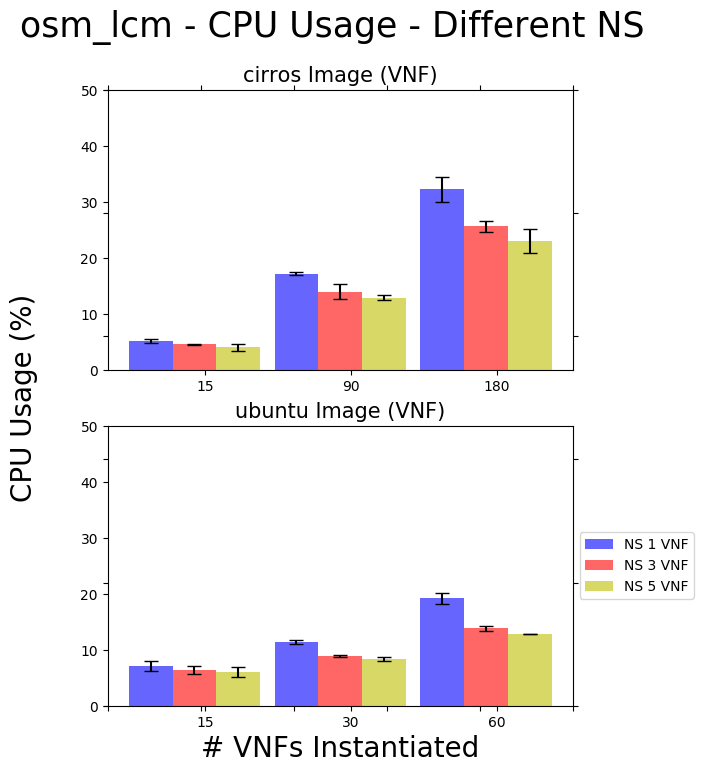
\includegraphics[width=0.7\linewidth]{figures/scalability_graphs/Docker-Grouped-Cases/osm/osm_lcm-Mean-CPU-Cases}
	\caption{}
	\label{fig:osmlcm-mean-cpu-cases}
\end{figure}

\begin{figure}[h]
	\centering
	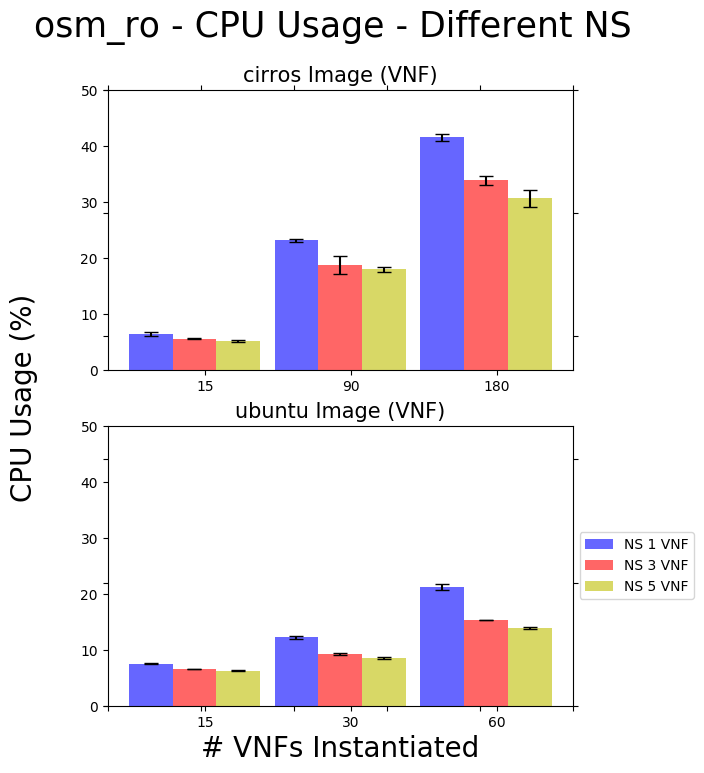
\includegraphics[width=0.7\linewidth]{figures/scalability_graphs/Docker-Grouped-Cases/osm/osm_ro-Mean-CPU-Cases}
	\caption{}
	\label{fig:osmro-mean-cpu-cases}
\end{figure}


\subsubsection{Container vs VM Orchestration} 

Container vs VM Orchestration

\begin{figure}[h]
	\centering
	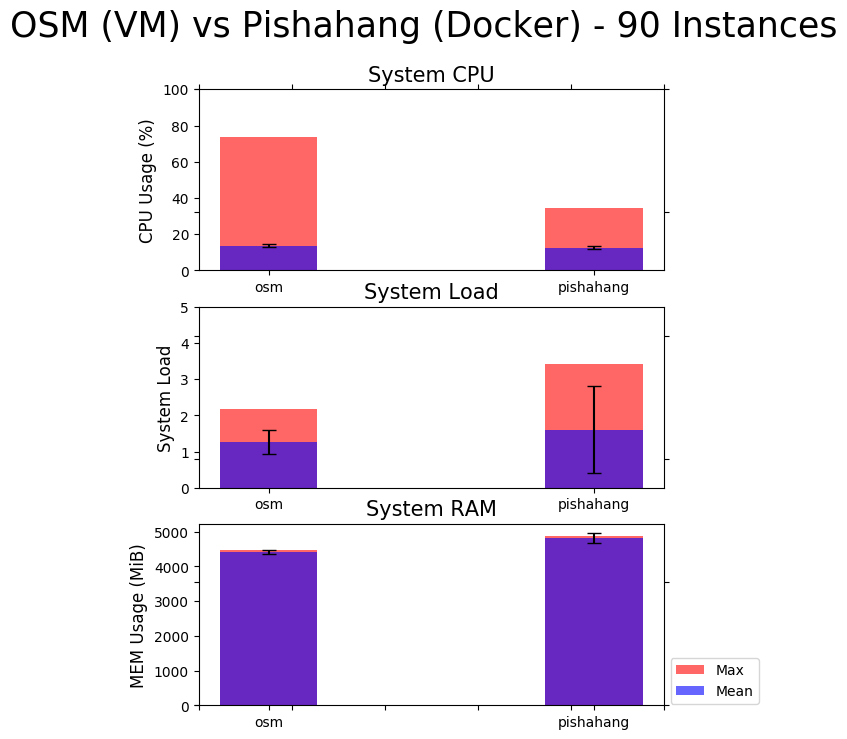
\includegraphics[width=0.7\linewidth]{figures/scalability_graphs/Comparison-VM-Docker/System_metrics_comparison}
	\caption{}
	\label{fig:systemmetricscomparison}
\end{figure}

\begin{figure}[h]
	\centering
	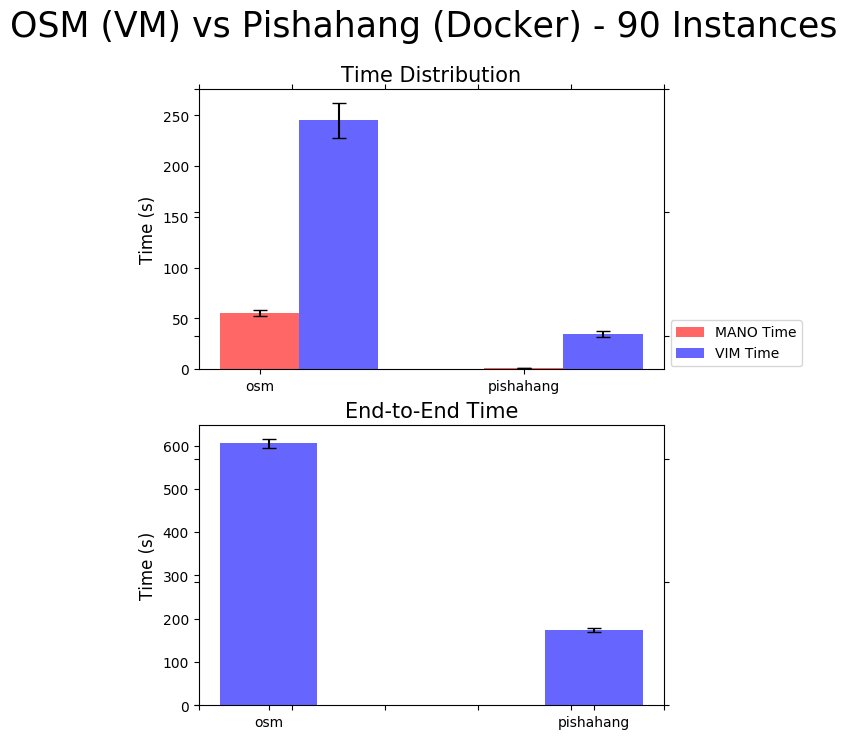
\includegraphics[width=0.7\linewidth]{figures/scalability_graphs/Comparison-VM-Docker/Time_comparison}
	\caption{}
	\label{fig:timecomparison}
\end{figure}


\subsubsection{Scaling Plugin Evaluation}

\begin{figure}[h]
	\centering
	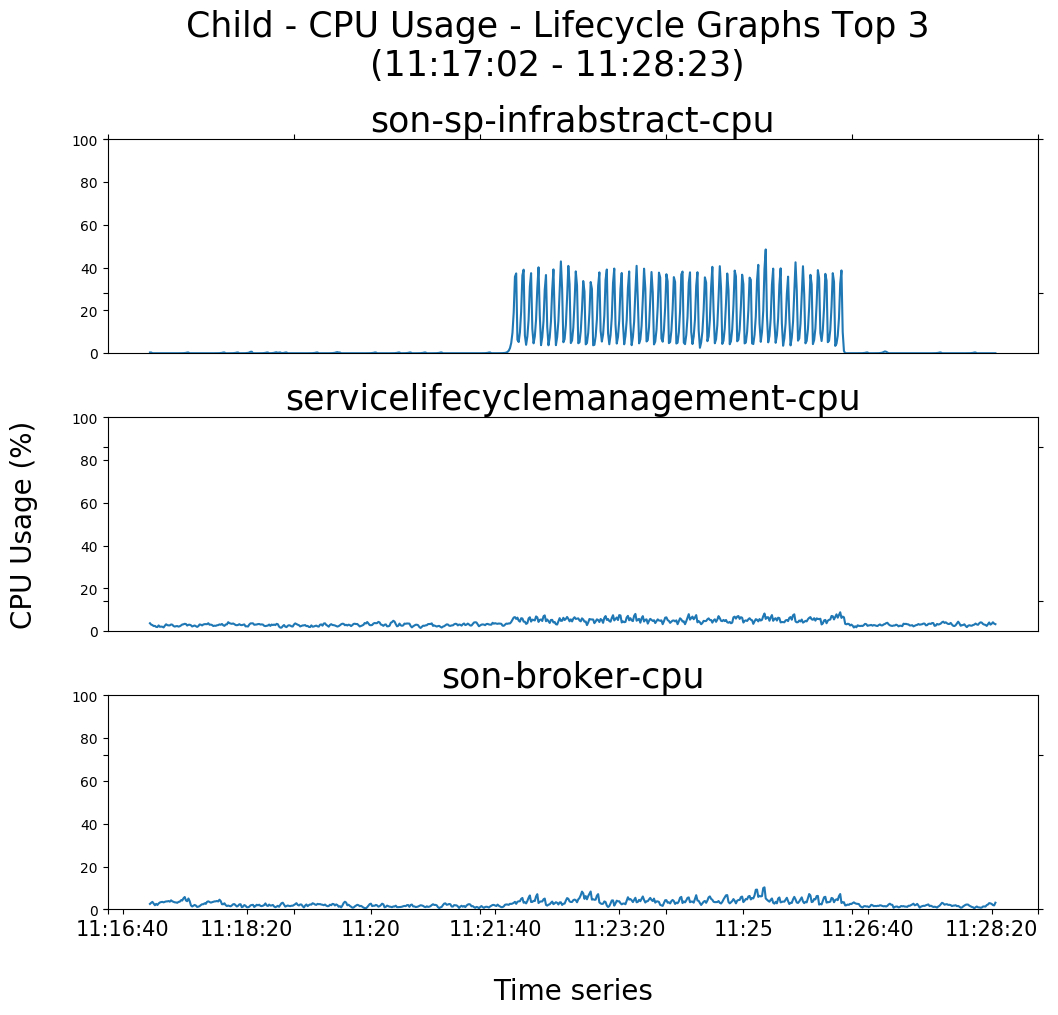
\includegraphics[width=0.7\linewidth]{figures/scalability_graphs/Scalability-Evaluation/Child-TOP-3-Lifecycle}
	\caption{Child scaling}
	\label{fig:child-top-3-lifecycle}
\end{figure}

\begin{figure}[h]
	\centering
	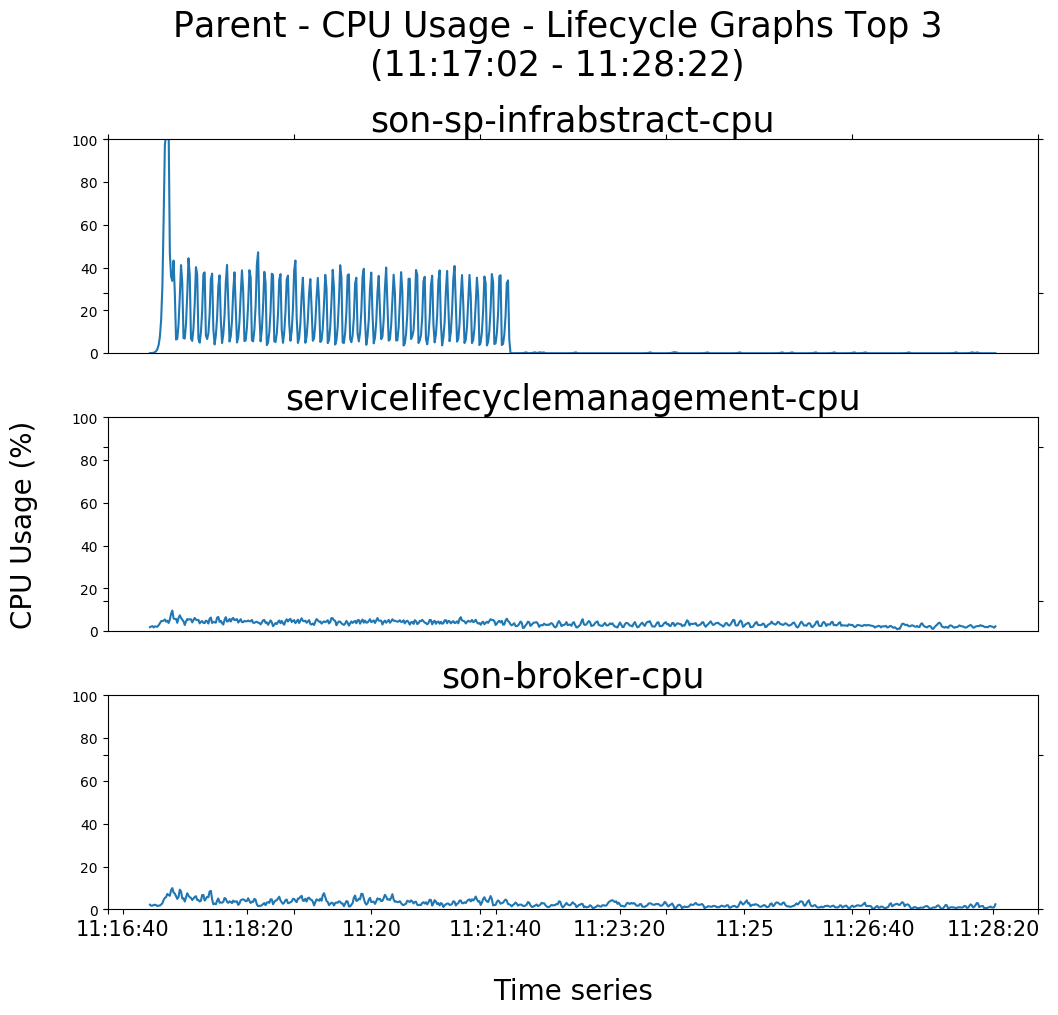
\includegraphics[width=0.7\linewidth]{figures/scalability_graphs/Scalability-Evaluation/Parent-TOP-3-Lifecycle}
	\caption{Parent Scaling}
	\label{fig:parent-top-3-lifecycle}
\end{figure}


\subsection{Future scope}